\documentclass{article}

% Remember to change this and recompile before use!
\def\today{<insert date>}
\def\lectureno{<insert lecture no>}
\def\classname{<insert class>}

\usepackage{amsmath}
\usepackage{amsthm}
\usepackage[utf8]{inputenc}
\usepackage[T1]{fontenc}
\usepackage{xcolor}
\usepackage{tikz}
\usepackage{tkz-euclide}
\usepackage{lmodern}
\usepackage[normalem]{ulem}
\usepackage{float}
\usepackage{fancyhdr}
\usepackage{microtype}
%\usepackage{showframe}
\usepackage{mdframed}
\usetikzlibrary{calc,intersections}
\tikzset{new/.style={color=red},small label/.style={font=\scriptsize},node label/.style={}}

\title{\classname \\ Length and Ratio} 
\author{T Yeung}
\date{\today}

\DeclareMathOperator{\Pow}{Pow}
\newtheorem{theorem}{Theorem}[section]
\newtheorem{corollary}{Corollary}[theorem]
\theoremstyle{definition}
\newtheorem{question}{Question}

\begin{document}
\pagestyle{fancy}
\fancyhead{}\fancyfoot{}
\fancyhead[L]{\classname}
\fancyhead[C]{L\lectureno}
\fancyhead[R]{\today}

\maketitle
\section{Trigonometric Identities}
Trigonometric identities simplify complex expressions.
\begin{equation*}
	\begin{split}
		1 &= \sin^2 \theta + \cos^2 \theta \\
		\sin(-\theta) &= - \sin \theta \\
		\cos(-\theta) &= \cos \theta \\
		\sin(\alpha + \beta) &= \sin \alpha \cos \beta + \sin \beta \cos \alpha \\ 
		\cos(\alpha + \beta) &= \cos \alpha \cos \beta - \sin \alpha \sin \beta \\
	\end{split}
\end{equation*}

By replacing $+$ with $-$ in $\sin(\alpha+\beta)$ and $\cos(\alpha+\beta)$, you get the other two identity. The four identities are collectively called the \emph{compound angle formula}. The proof of them is based on geometric construction.

By summing up the compound angle formulas in different ways, we obtain the product-to-sum identities.
\begin{equation*}
	\begin{split}
		2\cos \alpha \cos \beta &= \cos(\alpha - \beta) + \cos(\alpha + \beta) \\
		2\sin \alpha \sin \beta &= \cos(\alpha - \beta) - \cos(\alpha + \beta) \\
		2\sin \alpha \cos \beta &= \sin(\alpha - \beta) + \sin(\alpha + \beta)
	\end{split}
\end{equation*}

You can also derive the sum-to-product formulas by replacing $\alpha$ with  $\frac{\alpha+\beta}{2}$ and $\beta$ with  $\frac{\alpha-\beta}{2}$ in the above formulas.

\begin{equation*}
	\begin{split}
		\cos (a) \cos (b)&=\frac{1}{2}(\cos (a+b)+\cos (a-b) \\
		\sin (a) \sin (b)&=\frac{1}{2}(\cos (a-b)-\cos (a+b)) \\
		\sin (a) \cos (b)&=\frac{1}{2}(\sin (a+b)+\sin (a-b)) \\
	\end{split}
\end{equation*}

\section{The Extended Law Of Sine}

Recall the Extended Law of Sine we derived:

\begin{mdframed}
	\begin{theorem}[The Extended Law of Sine]
		Given a triangle $ABC$, we have 
		\begin{equation*}
			\frac{a}{\sin A} = \frac{b}{\sin B} = \frac{c}{\sin C} = 2\mathcal{R}
		\end{equation*}
	\end{theorem}
\end{mdframed}

We can use this result to prove the Ptolemy's Theorem.

\begin{mdframed}
	\begin{theorem}[Ptolemy's Theorem]
		Let $ABCD$ be a cyclic quadrilateral. Then
		\begin{equation*}
			AB \cdot CD + BC \cdot DA = AC \cdot BD
		\end{equation*}
	\end{theorem}
	\begin{figure}[H]
		\centering
		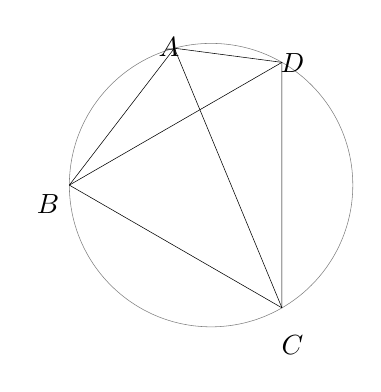
\begin{tikzpicture}[small label]
			\def\r{1.8}
			\tkzDefPoint(0,0){O}
			\tkzDefPoint(105:\r){A}
			\tkzDefPoint(60:\r){D}
			\tkzDefPoint(-60:\r){C}
			\tkzDefPoint(180:\r){B}
			\tkzDrawCircle(O,A)
			\tkzDrawPolygon(A,B,C,D)
			\tkzDrawSegments(A,C B,D)
			\tkzAutoLabelPoints[center=O](A,B,C,D)
			% Angle
		\end{tikzpicture}
		\caption{Statement of Ptolemy's Theorem}
	\end{figure}
\end{mdframed}
\begin{proof}
	Without loss of generality, we set $\mathcal{R} = \frac{1}{2}$ as the radius of $(ABCD)$.
	Let $AB = \sin \alpha_1$, $BC=\sin \alpha_2$, $CD=\sin \alpha_3$,  $DA=\sin \alpha_4$,
	$AC = \sin \angle ABC = \sin (\alpha_3 + \alpha_4)$,
	$BD = \sin \angle DAB = \sin(\alpha_2 + \alpha_3)$.
	 Note that by product-to-sum identities, we have
			\begin{equation*}
				\begin{split}
					\sin \alpha_1 \sin \alpha_3 &= \frac{1}{2}(\cos(\alpha_1	- \alpha_3) - \cos(\alpha_1 + \alpha_3)) \\
					\sin \alpha_2 \sin \alpha_4 &= \frac{1}{2}(\cos(\alpha_2-\alpha_4)-\cos(\alpha_2+\alpha_4)) \\
					\sin(\alpha_2+\alpha_3)\sin(\alpha_3+\alpha_4) &= \frac{1}{2}(\cos(\alpha_2-\alpha_4) - \cos(\alpha_2+2\alpha_3+\alpha_4))
				\end{split}
			\end{equation*}
	Since $\alpha_1 + \alpha_2 + \alpha_3 + \alpha_4 = 180^o$, we also have 
			\begin{equation*}
				\cos(\alpha_1+\alpha_3)+\cos(\alpha_2+\alpha_4)=0
			\end{equation*}
	Also note that
			\begin{equation*}
				\cos(\alpha_2+2\alpha_3+\alpha_4) = \cos(180^o-\alpha_1+\alpha_3)=-\cos(\alpha_1-\alpha_3)
			\end{equation*}
	The rest is trivial. :)
	\begin{figure}[H]
		\centering	
		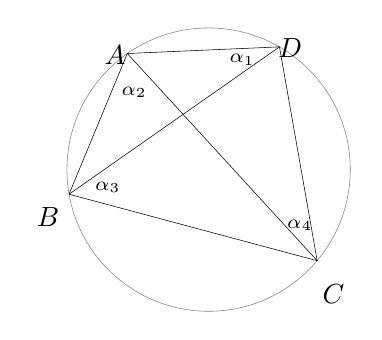
\begin{tikzpicture}[small label]
			\def\r{1.8}
			\tkzDefPoint(0,0){O}
			\tkzDefPoint(125:\r){A}
			\tkzDefPoint(60:\r){D}
			\tkzDefPoint(-40:\r){C}
			\tkzDefPoint(190:\r){B}
			\tkzDrawCircle(O,A)
			\tkzDrawPolygon(A,B,C,D)
			\tkzDrawSegments(A,C B,D)
			\tkzAutoLabelPoints[center=O](A,B,C,D)
			\tkzLabelAngle[small label,pos=0.5](A,D,B){$\alpha_1$}
			\tkzLabelAngle[small label,pos=0.5](B,A,C){$\alpha_2$}
			\tkzLabelAngle[small label,pos=0.5](C,B,D){$\alpha_3$}
			\tkzLabelAngle[small label,pos=0.5](D,C,A){$\alpha_4$}
		\end{tikzpicture}
		\caption{Proof of Ptolemy's Theorem}
	\end{figure}
\end{proof}

\begin{mdframed}
	\begin{corollary}[Stewart's Theorem]
		Let $ABC$ be a triangle. Let $D$ be a point on $\overline{BC}$ and let $m = DB$, $n = DC$, $d = AD$. Then
		\begin{equation*}
			a(d^2+mn)=b^2m+c^2n
		\end{equation*}
	\end{corollary}
	\begin{figure}[H]
		\centering
		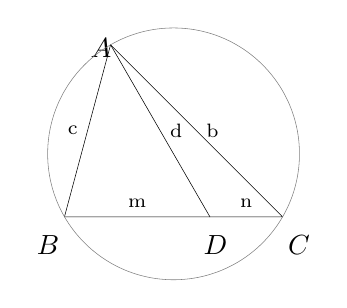
\begin{tikzpicture}[small label]
			\def\r{1.6}
			\tkzDefPoint(0,0){O}
			\tkzDefPoint(120:\r){A}
			\tkzDefPoint(210:\r){B}
			\tkzDefPoint(-30:\r){C}

			\tkzDefBarycentricPoint(B=1,C=2) \tkzGetPoint{D}
			\tkzDrawSegment(A,D)
			\tkzAutoLabelPoints[center=O](A,B,C,D)
			\tkzDrawPolygon(A,B,C)
			\tkzDrawCircle(O,A)
			\tkzLabelLine[left](A,B){c}
			\tkzLabelLine[right](A,D){d}
			\tkzLabelLine[right](A,C){b}
			\tkzLabelLine[above](B,D){m}
			\tkzLabelLine[above](D,C){n}
		\end{tikzpicture}
		\caption{Stewart's Theorem}
	\end{figure}
\end{mdframed}
	Often this is written in the form
	\begin{equation*}
		man + dad = bmb + cnc
	\end{equation*}
	as a mnemonic - "a \emph{man} and his \emph{dad} put a \emph{bomb} in the \emph{sink}".

	\begin{proof}
			Let $AD$ meet $(ABC)$ again at $P$.
			By similar triangle, we have $\frac{BP}{m} = \frac{b}{d}$ and $\frac{CP}{n} = \frac{c}{d}$.
			By Power Chord Theorem, we know that $DP = \frac{mn}{d}$.
			By Ptolemy's Theorem, we have
				$BC \cdot AP = AC \cdot BP + AB \cdot CP$
			. Hence,  $a\cdot (d+\frac{mn}{d}) = b\cdot \frac{bm}{d} + c \cdot \frac{cn}{d}$ which is the Stewart's Theorem.
		\begin{figure}[H]
			\centering
			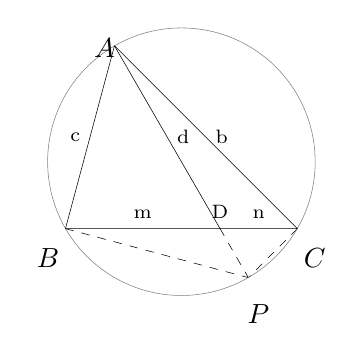
\begin{tikzpicture}[small label]
				\def\r{1.7}
				\tkzDefPoint(0,0){O}
				\tkzDefPoint(120:\r){A}
				\tkzDefPoint(210:\r){B}
				\tkzDefPoint(-30:\r){C}

				\tkzDefBarycentricPoint(B=1,C=2) \tkzGetPoint{D}
				\tkzInterLC(A,D)(O,A) \tkzGetSecondPoint{P}
				\tkzDrawSegment(A,D)
				\tkzDrawSegments[dashed](C,P D,P B,P)
				\tkzDrawCircle(O,A)
				\tkzDrawPolygon(A,B,C)
				\tkzAutoLabelPoints[center=O](A,B,C,P)
				\tkzLabelPoint[small label,above](D){D}
				\tkzLabelLine[left](A,B){c}
				\tkzLabelLine[right](A,D){d}
				\tkzLabelLine[right](A,C){b}
				\tkzLabelLine[above](B,D){m}
				\tkzLabelLine[above](D,C){n}
			\end{tikzpicture}
			\caption{Proof of Stewart's Theorem}
		\end{figure}
	\end{proof}

	Take a look at the following problem for another application of the Extended Law of Sine.
	\begin{question}
		(Prelim 2019 Q13) $A,B,C$ are three points on a circle while $P$ and $Q$ are two points on $AB$. The extensions of $CP$ and $CQ$ meet the circle at $S$ and $T$ respectively. If $AP=2$, $AQ=7$, $AB=11$, $AS=5$ and $BT=2$, find the length of $ST$.
	\end{question}
	\begin{figure}[H]
		\centering
		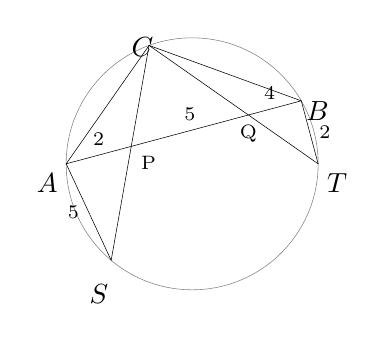
\begin{tikzpicture}[small label]
			\def\r{1.6}
			\tkzDefPoint(0,0){O}
			\tkzDefPoint(180:\r){A}
			\tkzDefPoint(30:\r){B}
			\tkzDefPoint(110:\r){C}
			\tkzDefPoint(230:\r){S}
			\tkzDefPoint(-0:\r){T}
			\tkzDrawCircle(O,A)
			\tkzDrawPolygon(A,B,C)
			\tkzDrawSegment(C,S)
			\tkzDrawSegment(C,T)
			\tkzDrawSegment(A,S)
			\tkzDrawSegment(B,T)
			\tkzInterLL(A,B)(C,S) \tkzGetPoint{P}
			\tkzInterLL(A,B)(C,T) \tkzGetPoint{Q}
			\tkzAutoLabelPoints[center=O](A,B,C,S,T)
			\tkzLabelPoint[small label,below right](P){P}
			\tkzLabelPoint[small label,below](Q){Q}
			\tkzLabelLine[above](A,P){2}
			\tkzLabelLine[above](P,Q){5}
			\tkzLabelLine[pos=0.4,above](Q,B){4}
			\tkzLabelLine[left](A,S){5}
			\tkzLabelLine[right](B,T){2}
		\end{tikzpicture}
		\caption{A not-to-scale diagram that is not provided in the contest}
	\end{figure}
	\newpage

\section{Angle Bisector Theorem}

\begin{mdframed}
	\begin{theorem}[Angle Bisector Theorem] Let $BD$ be the angle bisector of $\angle ABC$, then $AB:BC = AD:DC$.
	\end{theorem}
	\begin{figure}[H]
		\centering	
		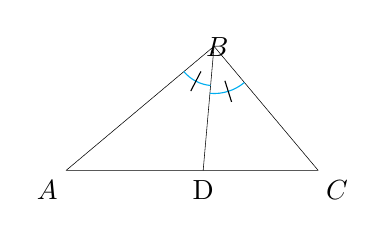
\begin{tikzpicture}
			\def\r{1.6}
			\tkzDefPoint(0,0){O}
			\tkzDefPoint(180:\r){A}
			\tkzDefPoint(80:\r){B}
			\tkzDefPoint(0:\r){C}
			\tkzDrawPolygon(A,B,C)
			\tkzDefLine[bisector](A,B,C) \tkzGetPoint{b}
			\tkzInterLL(B,b)(A,C) \tkzGetPoint{D}
			\tkzDrawSegment(B,D)
			\tkzAutoLabelPoints[center=O](A,B,C)
			\tkzLabelPoint[below](D){D}
			\tkzMarkAngle[size=0.5,cyan,mark=|](A,B,D)
			\tkzMarkAngle[size=0.6,cyan,mark=|](D,B,C)
		\end{tikzpicture}
	\end{figure}
\end{mdframed}
\begin{proof}
	By the Extended Law of Sine, we have $AB \cdot \sin \angle ABD \cdot DC = BC \cdot \sin \angle CBD \cdot AD$. Rearranging yields the Angle Bisector Theorem.
\end{proof}

\begin{question}
	(Prelim 2022 Q20) Let $ABCD$ be a cyclic quadrilateral and $E$ be the intersection of $AC$ and $BD$. $P$ and $Q$ are two points on $AC$ such that the points $A,E,Q,P,C$ lie on the same straight line in this order, and that $BP$ bisects $\angle ABC$ whereas $DQ$ bisects $\angle ADC$. If $AE=4$, $EQ=2$, and $QP=3$, find the length of $PC$.
\end{question}
\newpage

\subsection{Extended Angle Bisector Theorem}
We have the following extended version of the Angle Bisector Theorem

\begin{mdframed}
	\begin{theorem}[Extended Angle Bisector Theorem]
		Let $BD$ be the external angle bisector of $\angle ABC$, then $AB:BC = AD:DC$.
	\end{theorem}
	\begin{figure}[H]
		\centering
		\begin{tikzpicture}
			\def\r{1.6}
			\tkzDefPoint(0,0){O}
			\tkzDefPoint(180:\r){A}
			\tkzDefPoint(130:\r){B}
			\tkzDefPoint(0:\r){C}
			\coordinate (E) at ($(C)!1.4!(B)$);
			\tkzDefLine[bisector](E,B,A) \tkzGetPoint{b}
			\tkzInterLL(B,b)(A,C) \tkzGetPoint{D}
			\tkzLabelPoint[below](A){A}
			\tkzLabelPoint[right](C){C}
			\tkzLabelPoint[above](B){B}
			\tkzLabelPoint[left](D){D}
			\tkzDrawSegment(A,B)
			\tkzDrawSegment(E,C)
			\tkzDrawSegment(C,D)
			\tkzDrawSegment(B,D)
			\tkzMarkAngle[size=0.6,cyan,mark=|](D,B,A)
			\tkzMarkAngle[size=0.5,cyan,mark=|](E,B,D)
		\end{tikzpicture}
	\end{figure}
\end{mdframed}
\begin{proof}
	Left as an exercise.
\end{proof}
\vspace{4cm}
\begin{question}
	(Prelim 2022 Q19) In $\triangle A B C, A B<A C$. The internal bisector of $\angle B A C$ meets $B C$ at $D$, while the external bisector of $\angle B A C$ meets $C B$ produced at $E$. If $EB=10$ and $BD=5$, find the length of $DC$.
\end{question}

\newpage

\section{Cosine's Law}
\begin{mdframed}
	\begin{theorem}[Cosine's Law]
		In $\triangle ABC$,  $c^2 = a^2 + b^2 - 2ab\cos C$. Equivalently, $\cos C = \frac{a^2+b^2-c^2}{2ab}$
	\end{theorem}
\end{mdframed}
\begin{proof}
	Observe that $c^2=AH^2+HB^2=b\sin C^2+(a-b\cos C)^2=a^2+b^2-2ab\cos C$.
	\begin{figure}[H]
		\centering
		\begin{tikzpicture}
			\tkzDefPoint(-1,0){A}		
			\tkzDefPoint(2,0){B}		
			\tkzDefPoint(0,1){C}		
			\tkzDrawPolygon(A,B,C)
			\tkzDefPointBy[projection=onto A--B](C) \tkzGetPoint{H}
			\tkzLabelPoint[left](A){C}
			\tkzLabelPoint[right](B){B}
			\tkzLabelPoint[above](C){A}
			\tkzLabelPoint[below](H){H}
			\tkzDrawSegment(C,H)
		\end{tikzpicture}
		\caption{Proof of Cosine's Law}
	\end{figure}
\end{proof}
\begin{question}
	Prove the Stewart's Theorem with the Cosine's Law.
\end{question}
\vspace{5cm}
\section{Ceva's Theorem}
In a triangle, a \emph{cevian} is a line joining a vertex of a triangle to a point on the interior of the opposite side. A natural question is when three cevians of a triangle concurs. This is answered by Ceva's theorem.
\begin{mdframed}
	\begin{theorem}[Ceva's Theorem]
		Let $\overline{AX}$,  $\overline{BY}$,  $\overline{CZ}$ be cevians of a triangle $ABC$. They concur if and only if
		\begin{equation*}
			\frac{BX}{XC} \cdot \frac{CY}{YA} \cdot \frac{AZ}{ZB} = 1
		\end{equation*}
		\begin{figure}[H]
			\centering
			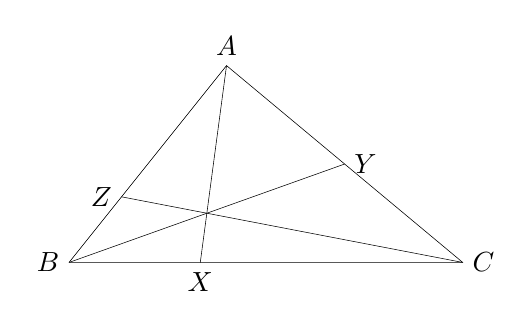
\begin{tikzpicture}
				\tkzDefPoint(0,0){A}
				\tkzDefPoint(-2,-2.5){B}
				\tkzDefPoint(3,-2.5){C}
				\coordinate (X) at ($(B)!0.333333333333!(C)$);
				\coordinate (Z) at ($(B)!0.333333333333!(A)$);
				\coordinate (Y) at ($(C)!0.5!(A)$);
				\tkzDrawPolygon(A,B,C)
				\tkzDrawSegment(A,X)
				\tkzDrawSegment(B,Y)
				\tkzDrawSegment(C,Z)
				\tkzLabelPoints[above](A){A}
				\tkzLabelPoints[left](B){B}
				\tkzLabelPoints[right](C){C}
				\tkzLabelPoints[below](X){X}
				\tkzLabelPoints[right](Y){Y}
				\tkzLabelPoints[left](Z){Z}
			\end{tikzpicture}
			\caption{Statement of Ceva's Theorem}
		\end{figure}
	\end{theorem}
\end{mdframed}
\begin{proof}
	Observe that $\frac{[ABX]}{[AXC]} = \frac{BX}{XC}$ and $\frac{[BPX]}{[CPX]} = \frac{BX}{XC}$.
	Hence $\frac{[APB]}{[APC]} = \frac{BX}{XC}$.
	Similarly $\frac{[BPA]}{[BPC]} = \frac{AY}{YC}$ and  $\frac{[CPB]}{[CPA]} = \frac{ZB}{ZA}$.
	Multiplying the above three equations gives $\frac{BX}{XC} \cdot \frac{CY}{YA} \cdot \frac{AZ}{ZB} = 1$.
	\begin{figure}[H]
		\centering
		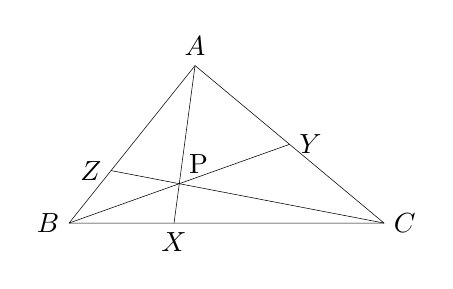
\begin{tikzpicture}[scale=0.8]
			\tkzDefPoint(0,0){A}
			\tkzDefPoint(-2,-2.5){B}
			\tkzDefPoint(3,-2.5){C}
			\coordinate (X) at ($(B)!0.333333333333!(C)$);
			\coordinate (Z) at ($(B)!0.333333333333!(A)$);
			\coordinate (Y) at ($(C)!0.5!(A)$);
			\tkzDrawPolygon(A,B,C)
			\tkzDrawSegment(A,X)
			\tkzDrawSegment(B,Y)
			\tkzDrawSegment(C,Z)
			\tkzLabelPoints[above](A){A}
			\tkzLabelPoints[left](B){B}
			\tkzLabelPoints[right](C){C}
			\tkzLabelPoints[below](X){X}
			\tkzLabelPoints[right](Y){Y}
			\tkzLabelPoints[left](Z){Z}
			\tkzInterLL(A,X)(B,Y) \tkzGetPoint{P}
			\tkzLabelPoint[above right](P){P}
		\end{tikzpicture}
		\caption{Proof of Ceva's Theorem}
	\end{figure}
\end{proof}

The above proof only proves the forward direction, i.e., if three points concurs, then the ratio must comply with the equation; The backward direction is also true, i.e., if the ratio complies with the equation, then three points concur. However, the proof is not given here since the technique is not very helpful for short-answer contest.

\begin{mdframed}
	\begin{theorem}[Trigonometric Form of Ceva's Theorem]
		Let $\overline{AX}$,  $\overline{BY}$,  $\overline{CZ}$ be cevians of a triangle  $ABC$. They concur if and only if
		\begin{equation*}
			\frac{\sin \angle BAX \sin \angle CBY \sin \angle ACZ}{\sin \angle XAC \sin \angle YBA \sin \angle ZCB } = 1
		\end{equation*}
	\end{theorem}
	\begin{figure}[H]
		\centering
		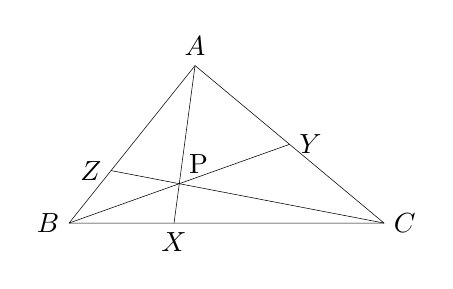
\begin{tikzpicture}[scale=0.8]
			\tkzDefPoint(0,0){A}
			\tkzDefPoint(-2,-2.5){B}
			\tkzDefPoint(3,-2.5){C}
			\coordinate (X) at ($(B)!0.333333333333!(C)$);
			\coordinate (Z) at ($(B)!0.333333333333!(A)$);
			\coordinate (Y) at ($(C)!0.5!(A)$);
			\tkzDrawPolygon(A,B,C)
			\tkzDrawSegment(A,X)
			\tkzDrawSegment(B,Y)
			\tkzDrawSegment(C,Z)
			\tkzLabelPoints[above](A){A}
			\tkzLabelPoints[left](B){B}
			\tkzLabelPoints[right](C){C}
			\tkzLabelPoints[below](X){X}
			\tkzLabelPoints[right](Y){Y}
			\tkzLabelPoints[left](Z){Z}
			\tkzInterLL(A,X)(B,Y) \tkzGetPoint{P}
			\tkzLabelPoint[above right](P){P}
		\end{tikzpicture}
		\caption{Trigonometric Form of Ceva's Theorem}
	\end{figure}
\end{mdframed}
\begin{proof}
	Use the Extended Law of Sine. Left as an exercise.
\end{proof}

\subsection{Existence of orthocenter, incenter, centroid}
If you have two altitudes, they obviously meet at the same point. However, why does the third altitude necessarily pass through the intersection of the first and second altitudes? 

This is given by the Ceva's Theorem. We only need to check
	\begin{equation*}
		\frac{\sin(90^o-B)\sin(90^o-C)\sin(90^o-A)}{\sin(90^o-C)\sin(90^o-A)\sin(90^o-B)} = 1
	\end{equation*}
Hence, the orthocentre exists.

Similar calculations show that the incenter exists:
\begin{equation*}
	\frac{\sin \frac{1}{2}A \sin \frac{1}{2}B \sin \frac{1}{2}C}{\sin \frac{1}{2}A \sin \frac{1}{2}B \sin \frac{1}{2}C} = 1
\end{equation*}

Alternatively, we can use the normal form of Ceva's Theorem together with the Angle Bisector Theorem to show that the incenter exists.

Lastly, the existence of centroid is trivial with the help of Ceva's Theorem.
\begin{equation*}
	\frac{1}{1} \frac{1}{1} \frac{1}{1} = 1
\end{equation*}

\section{Menelaus's Theorem}
\begin{mdframed}
	\begin{theorem}[Menelaus's Theorem]
		Let $X$, $Y$, $Z$ be points on lines $BC$, $CA$, $AB$ in a triangle $ABC$, distinct from its vertices. Then $X$, $Y$, $Z$ are collinear (if and only if
		\begin{equation*}
			\frac{BX}{XC} \cdot \frac{CY}{YA} \cdot \frac{AZ}{ZB} = -1
		\end{equation*}
		where lengths are directed.
	\end{theorem}
	\begin{figure}[H]
		\centering
		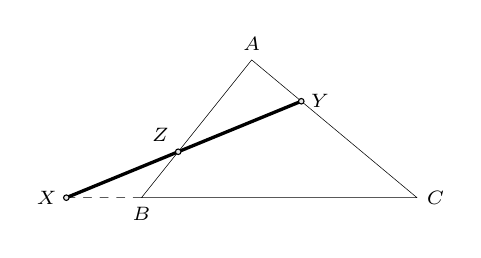
\begin{tikzpicture}[scale=0.7,small label]
			\tkzDefPoint(0,0){A}
			\tkzDefPoint(-2,-2.5){B}
			\tkzDefPoint(3,-2.5){C}
			\coordinate (Z) at ($(B)!0.333333333333!(A)$);
			\coordinate (Y) at ($(C)!0.7!(A)$);
			\tkzInterLL(Z,Y)(B,C) \tkzGetPoint{X}
			\tkzDrawPolygon(A,B,C)
			\tkzLabelPoints[small label,above](A){A}
			\tkzLabelPoints[small label,below](B){B}
			\tkzLabelPoints[small label,right](C){C}
			\tkzLabelPoints[small label,left](X){X}
			\tkzLabelPoints[small label,right](Y){Y}
			\tkzLabelPoints[small label,above left](Z){Z}
			\tkzDrawSegment[very thick](X,Y)
			\tkzDrawSegment[dashed](B,X)
			\tkzDrawPoints(X,Z,Y)
		\end{tikzpicture}
		\begin{tikzpicture}[scale=0.5,small label]
			\tkzDefPoint(1,0){A}
			\tkzDefPoint(-0.5,-2.5){B}
			\tkzDefPoint(3,-2.5){C}
			\coordinate (Z) at ($(B)!2!(A)$);
			\tkzInterLL(X,Z)(A,C) \tkzGetPoint{Y}
			\tkzInterLL(Z,Y)(B,C) \tkzGetPoint{X}
			\tkzDrawPolygon(A,B,C)
			\tkzLabelPoints[small label,above](A){A}
			\tkzLabelPoints[small label,below](B){B}
			\tkzLabelPoints[small label,right](C){C}
			\tkzLabelPoints[small label,left](X){X}
			\tkzLabelPoints[small label,left](Y){Y}
			\tkzLabelPoints[small label,above left](Z){Z}
			\tkzDrawSegment[very thick](X,Z)
			\tkzDrawSegment[dashed](B,X)
			\tkzDrawSegment[dashed](A,Y)
			\tkzDrawSegment[dashed](A,Z)
			\tkzDrawPoints(X,Z,Y)
		\end{tikzpicture}
		\caption{Statement of Menelaus's Theorem}
	\end{figure}
\end{mdframed}
\begin{proof}
	 Drop a perpendicular line from $A$ to $A'$, $B$ to $B'$, $C$ to $C'$ on $XY$.
	 We have $\frac{CY}{YA} = \frac{CC'}{AA'}$, $\frac{AA'}{BB'} = \frac{AZ}{ZB}$, and $\frac{BX}{XC} = -\frac{BB'}{CC'}$.
	 Multiplying all of them gives the Menelaus's Theorem.
	\begin{figure}[H]
			\centering
			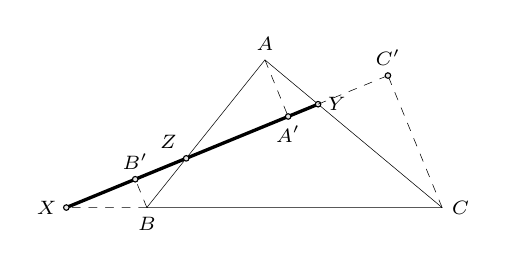
\begin{tikzpicture}[scale=0.75,small label]
				\tkzDefPoint(0,0){A}
				\tkzDefPoint(-2,-2.5){B}
				\tkzDefPoint(3,-2.5){C}
				\coordinate (Z) at ($(B)!0.333333333333!(A)$);
				\coordinate (Y) at ($(C)!0.7!(A)$);
				\tkzInterLL(Z,Y)(B,C) \tkzGetPoint{X}
				\tkzDrawPolygon(A,B,C)
				\tkzLabelPoints[small label,above](A){A}
				\tkzLabelPoints[small label,below](B){B}
				\tkzLabelPoints[small label,right](C){C}
				\tkzLabelPoints[small label,left](X){X}
				\tkzLabelPoints[small label,right](Y){Y}
				\tkzLabelPoints[small label,above left](Z){Z}
				\tkzDrawSegment[very thick](X,Y)
				\tkzDrawSegment[dashed](B,X)
				\tkzDrawPoints(X,Z,Y)
				\tkzDefPointBy[projection=onto X--Y](A) \tkzGetPoint{A'}
				\tkzDefPointBy[projection=onto X--Y](B) \tkzGetPoint{B'}
				\tkzDefPointBy[projection=onto X--Y](C) \tkzGetPoint{C'}
				\tkzDrawSegments[dashed](A,A' B,B' C,C')
				\tkzDrawSegment[dashed](Y,C')
				\tkzLabelPoints[small label](A')
				\tkzLabelPoints[small label,above](B')
				\tkzLabelPoints[small label,above](C')
				\tkzDrawPoints(B',A',C')
			\end{tikzpicture}
			\caption{Proof of Menelaus's Theorem}
		\end{figure}
\end{proof}

\section{The Centroid Triangle}
\begin{mdframed}
	\begin{theorem}[The Median Division]
		The medians divides the triangle into $6$ equal parts.
	\end{theorem}
	\begin{figure}[H]
		\centering
		\begin{tikzpicture}[small label,scale=1.1]
			\tkzDefPoint(0.5,0.5){A}
			\tkzDefPoint(-2,-1.5){B}
			\tkzDefPoint(1,-1.5){C}
			\tkzDrawPolygon(A,B,C)
			\tkzDefCentroid(A,B,C) \tkzGetPoint{G}
			\tkzInterLL(A,G)(B,C) \tkzGetPoint{M}
			\tkzInterLL(B,G)(A,C) \tkzGetPoint{N}
			\tkzInterLL(C,G)(A,B) \tkzGetPoint{L}
			\tkzDrawSegment(A,M)
			\tkzDrawSegment(B,N)
			\tkzDrawSegment(C,L)
			\tkzLabelPoint[small label,above](G){G}
			\tkzLabelPoint[small label,left](B){B}
			\tkzLabelPoint[small label,right](C){C}
			\tkzLabelPoint[small label,above](A){A}
			\tkzLabelPoint[small label,below](M){M}
			\tkzLabelPoint[small label,right](N){N}
			\tkzLabelPoint[small label,left](L){L}
		\end{tikzpicture}
		\caption{Statement of Centroid Division}
	\end{figure}
\end{mdframed}
\begin{proof}
	Left as an exercise (hint: Consider ratio of areas).
\end{proof}
\begin{question}
	(Centroid Division) Show that $AG=2GM$.
\end{question}

\section{Practice Problems}
	\begin{question}
		Point $P$ is on side $AB$ of right angled $\triangle ABC$ with $B$ as the right angled. Point $Q$ is on $AC$ such that $PQ$ is perpendicular to $AC$. It is given that $BC=3$ and $BP=PA=2$. Find the length $BQ$.
	\end{question}	
	\vfill
	\begin{question}
		(Prelim 2020 Q16) $\triangle ABC$ is right-angled at $B$, with $AB=1$ and $BC=3$. $E$ is the foot of perpendicular from $B$ to $AC$. $BA$ and $BE$ are produced to $D$ and $F$ respectively such that $D$,$F$,$C$ are collinear and $\angle DAF = \angle BAC$. Find the length of $AD$.
	\end{question}
	\vfill
	\newpage
	\begin{question}
		(Prelim 2019 Q10)	In $\triangle ABC$, $AB < AC$. Let $H$ be the orthocentre of $\triangle ABC$, and  $D$ be the foot of the perpendicular from $A$ to $BC$. If $AH=4$,$HD=3$ and $BC=12$, find the length of $BD$.
	\end{question}

\end{document}

